\documentclass[runningheads]{llncs}
%
\usepackage{graphicx}
\usepackage{xtab}
\usepackage{stmaryrd}
\usepackage{amsmath, amssymb}
\usepackage{listings}
% If you use the hyperref package, please uncomment the following line
% to display URLs in blue roman font according to Springer's eBook style:
% \renewcommand\UrlFont{\color{blue}\rmfamily}
\allowdisplaybreaks

% OUR MACROS
%%%%%%%%%%%%%%%%%%%%%%%%%%%%%%%%%%%%%%%%%%%%%%
%							References
%%%%%%%%%%%%%%%%%%%%%%%%%%%%%%%%%%%%%%%%%%%%%%

\newcommand{\chapref}[1]{Chapter~\ref{#1}}
\newcommand{\appref}[1]{Appendix~\ref{#1}}
\newcommand{\sectref}[1]{Section~\ref{#1}}
\newcommand{\subsectref}[1]{Subsection~\ref{#1}}
\newcommand{\figref}[1]{Figure~\ref{#1}}
\newcommand{\tabref}[1]{Table~\ref{#1}}
\newcommand{\egref}[1]{Example~\ref{#1}}
\newcommand{\eqnref}[1]{(\ref{#1})}
\newcommand{\thmref}[1]{Theorem~\ref{#1}}
\newcommand{\propref}[1]{Proposition~\ref{#1}}
\newcommand{\lemref}[1]{Lemma~\ref{#1}}
\newcommand{\defref}[1]{Definition~\ref{#1}}

\newcommand{\chapchapref}[2]{Chapters~\ref{#1} and \ref{#2}}
\newcommand{\sectsectref}[2]{Sections~\ref{#1} and \ref{#2}}
\newcommand{\figfigref}[2]{Figures~\ref{#1} and \ref{#2}}
\newcommand{\tabtabref}[2]{Tables~\ref{#1} and \ref{#2}}

\newcommand{\sectsectsectref}[3]{Sections~\ref{#1}, \ref{#2} and \ref{#3}}
\newcommand{\figfigfigref}[3]{Figures~\ref{#1}, \ref{#2} and \ref{#3}}

%%%%%%%%%%%%%%%%%%%%%%%%%%%%%%%%%%%%%%%%%%%%%%
%							Code Listings
%%%%%%%%%%%%%%%%%%%%%%%%%%%%%%%%%%%%%%%%%%%%%%

%% Core language
%\lstdefinelanguage{SaltyLang}{
% keywords=[1]{all, any, mutex}
% keywordstyle[1]=\color{Cyan},
% keywords=[2]{controller, where, input, output, enum, env_init, env_trans, env_liveness, sys_init, sys_trans, sys_liveness, def},
% keywordstyle=[2]\color{blue!90!black},%\bfseries,
% keywords=[3]{False, True},
% keywordstyle=[3]\color{ForestGreen},%\bfseries,
% keywords=[4]{all, any, mutex, leads_to, Bool, if, then, else},
% keywordstyle=[4]\color{Cyan},
% otherkeywords={', !, <, ->, <->, \, /, /\\, \\/},
% keywordstyle=\color{Cyan},
% identifierstyle=\color{black},
% sensitive=true,
% comment=[l]{--},
% commentstyle=\color{Magenta}
%}
%
%% Additional options
%\lstset{
% language=SaltyLang,
% basicstyle=\small\ttfamily,
% tabsize = 2,
% numbers=none,
% mathescape=false,
% showstringspaces=false
%}

%%%%%%%%%%%%%%%%%%%%%%%%%%%%%%%%%%%%%%%%%%%%%%
%							Theorem Environments
%%%%%%%%%%%%%%%%%%%%%%%%%%%%%%%%%%%%%%%%%%%%%%

%\newtheorem{lemma}{Lemma}
%\theoremstyle{definition} % turn off pesky italics
%\newtheorem{definition}{Definition}
%\newtheorem{example}{Example}
%\newtheorem{theorem}{Theorem}
%\newtheorem{proposition}{Proposition}
%\newtheorem{proof}{Proof}


%%%%%%%%%%%%%%%%%%%%%%%%%%%%%%%%%%%%%%%%%%%%%%
%							Definitions
%%%%%%%%%%%%%%%%%%%%%%%%%%%%%%%%%%%%%%%%%%%%%%

% Standard sets of numbers
\def\Nset{\mathbb{N}}
\def\Rset{\mathbb{R}}
\def\Zset{\mathbb{Z}}

% Reactive synthesis sets
\def\inputs{\mathcal{I}}
\def\outputs{\mathcal{O}}


% abbreviations
%\def\act{{Act}}
%\def\sinit{{\overline{s}}}

% logical operators
\def\limplies{\rightarrow}
\newcommand{\lequiv}{\leftrightarrow}
\newcommand{\ltrue}{\textrm{true}}
\newcommand{\lfalse}{\textrm{false}}
\newcommand{\lxor}{\oplus}

% temporal operators
\def\always{\square}
\def\until{\mathbin{\mathsf{U}}}
\def\wuntil{\mathbin{\mathsf{W}}}
\def\release{\mathbin{\mathsf{R}}}
\def\eventually{\lozenge}
\def\always{\square}
\def\lnext{\varbigcirc}

\def\palways{\square^{-1}}
\def\peventually{\lozenge^{-1}}
\def\past{\varbigcirc^{-1}}

\newcommand{\talways}[2]{\square^{#1..#2}}
\newcommand{\teventually}[2]{\lozenge^{#1..#2}}
\newcommand{\tuntil}[2]{\mathbin{\mathsf{U}}^{#1..#2}}
\newcommand{\trelease}[2]{\mathbin{\mathsf{R}}^{#1..#2}}


% model checking

%\def\true{{\mathit{true}}}
%\def\false{{\mathit{false}}}
%\def\AP{{\mathit{AP}}}
%\def\Dist{{\mathit{Dist}}}
%\def\Sat{{\mathit{Sat}}}
%\def\Steps{{\mathit{Steps}}}
%\def\sinit{{s_\mathit{init}}}
%\def\Prob{{\mathit{Prob}}}
%\def\Pr{{\mathit{Pr}}}
%\def\Path{{\mathit{Path}}}
%\def\Pathfin{{\mathit{FPath}}}
%\def\Pathful{{\mathit{Path}_\mathit{ful}}}
%\def\Adv{{\mathit{Adv}}}
%\def\calAfair{{{\cal A}_\mathit{fair}}}
%\def\sat{{\,\models\,}}
%\def\notsat{{\,\not\models\,}}
%\def\satAdv{{\,\models_\mathit{Adv}\,}}
%\def\notsatAdv{{\,\not\models_\mathit{Adv}\,}}
%\def\satfair{{\,\models_\mathit{fair}\,}}
%\def\next{{X\,}}
%\def\until{{\ {\cal U}\ }}
%\def\buntil{{\ {\cal U}^{\leq k}\ }}
%\def\tuntil{{\ {\cal U}^{\leq t}\ }}
%\def\sqlt{{\sqsubset}}
%\def\sqleq{{\sqsubseteq}}
%\def\sqgt{{\sqsupset}}
%\def\sqgeq{{\sqsupseteq}}
%\def\psmin{{p_s^\mathit{min}}}
%\def\psmax{{p_s^\mathit{max}}}
%\def\ptmin{{p_t^\mathit{min}}}
%\def\ptmax{{p_t^\mathit{max}}}
%\def\pspmin{{p_{s'}^\mathit{min}}}
%\def\pspmax{{p_{s'}^\mathit{max}}}
%\def\Syes{{S^{\mathit{yes}}}}
%\def\Sno{{S^{\mathit{no}}}}
%\def\Sqm{{S^?}}
%\def\done{{\mathit{done}}}
%\def\calPbp{{\cal P}_{\bowtie p}}
%\def\calSbp{{\cal S}_{\bowtie p}}
%\def\Var{{\mathit{Var}}}
%\def\Act{{\mathit{Act}}}
%\def\glob{{\mathit{glob}}}
%\def\ind{{\mathit{ind}}}
%\def\enc{{\mathit{enc}}}
%\def\etmcc{{ $\mathsf{E} {\;} \rotatebox{90}{$\mathsf{T}$} {\;} \mathsf{MC}^\mathsf{2}$ }}
%\def\implies{{\rightarrow}}

%%%%%%%%%%%%%%%%%%%%%%%%%%%%%%%%%%%%%%%%%%%%%%
%							Commands
%%%%%%%%%%%%%%%%%%%%%%%%%%%%%%%%%%%%%%%%%%%%%%


\newcommand{\pdist}[1]{\mathcal{D}({#1})}
\newcommand{\tfunction}{\longrightarrow}
\newcommand{\trans}[3]{#1 \overset{#2}{\longrightarrow} #3}
\newcommand{\allstates}{\overline{S}}

\newcommand{\allstratstwo}{\Sigma}
\newcommand{\strattwo}{\sigma}
\newcommand{\Rsetinf}{\Rset_{\pm\infty}}
\def\Rset{\mathbb{R}}
\def\Qset{\mathbb{Q}}
\newcommand{\dwc}{\textsf{dwc}}
\newcommand{\mydef}{\stackrel{\mbox{\rm {\tiny def}}}{=}}
\newcommand{\PONE}[1]{\textsf{Player~1}}
\newcommand{\PTWO}[1]{\textsf{Player~2}}
\newcommand{\PLAYER}[1]{\textsf{Player}~${#1}$}
\newcommand{\Exp}{\mathbb{E}}
%\renewcommand{\Pr}{\mathrm{Pr}}
\newcommand{\rew}{\mathsf{rew}}


\def\calPle{{\cal P}_{\le \lambda}}
\def\Pr{{\mathit{Pr}}}
\def\Prps{{\mathit{Pr}_{M^c}^{\sinit}}}


\newcommand{\salty}{Salty\xspace}
\newcommand{\enum}{{\texttt{enum}}\xspace}
\newcommand{\true}{{\texttt{True}}\xspace}
\newcommand{\false}{{\texttt{False}}\xspace}
\newcommand*\necessary{\mathord{\Box}}
\newcommand*\possible{\mathord{\Diamond}}
\newcommand{\sysinit}{\lstinline{sys_init}\xspace}%{{\texttt{sys\_init}}\xspace}
\newcommand{\envinit}{\lstinline{env_init}\xspace}%{{\texttt{env\_init}}\xspace}
\newcommand{\systrans}{\lstinline{sys_trans}\xspace}%{{\texttt{sys\_trans}}\xspace}
\newcommand{\envtrans}{\lstinline{env_trans}\xspace}%{{\texttt{env\_trans}}\xspace}
\newcommand{\sysliveness}{\lstinline{sys_liveness}\xspace}%{{\texttt{sys\_liveness}}\xspace}
\newcommand{\envliveness}{\lstinline{env_liveness}\xspace}%{{\texttt{env\_liveness}}\xspace}


\begin{document}
\lstset{language=Ada}
\lstset{basicstyle=\ttfamily}
%%%%%%%%%%%%%%%%%%%%%%%%%%%%%%%%%%%%%%%%%%%%%%%%%%%%%%%%%%%%%%%%%%%%%%%%%%%%%%%%
% TITLE
%%%%%%%%%%%%%%%%%%%%%%%%%%%%%%%%%%%%%%%%%%%%%%%%%%%%%%%%%%%%%%%%%%%%%%%%%%%%%%%%
%
\title{\large End-to-End Verification of Initial and Transition Properties of GR(1) Designs in SPARK}

%\thanks{Supported by AFRL contract FA8650-16-C-2642 and AFOSR grant RQCOR20-35.}}
%
\titlerunning{End-to-End Verification of GR(1) Designs in SPARK}
% If the paper title is too long for the running head, you can set
% an abbreviated paper title here
%
\author{Author 1\inst{1} \and
Author 2\inst{2} \and
Author 3\inst{3}}

%\author{Laura Humphrey\inst{1} \and
%James Hamil\inst{2} \and
%Joffrey Huguet\inst{3}}
%

% \authorrunning{L. Humphrey et al.}
\authorrunning{Author 1 et al.}

% First names are abbreviated in the running head.
% If there are more than two authors, 'et al.' is used.
%
\institute{Institute 1 \\
\email{author1@email.com} \and
Institute 2 \\
\email{author2@email.com}  \and
Institute 3 \\
 \email{author3@email.com}}
%
%\institute{Air Force Research Laboratory, WPAFB, OH 45433, USA \\
%\email{laura.humphrey@us.af.mil} \and
%LinQuest Corp., Beavercreek, OH 45431, USA \\
%\email{james.hamil.ctr@us.af.mil}  \and
%AdaCore, F-75009 Paris, France \\
% \email{huguet@adacore.com}}
%
\maketitle              % typeset the header of the contribution
%
%%%%%%%%%%%%%%%%%%%%%%%%%%%%%%%%%%%%%%%%%%%%%%%%%%%%%%%%%%%%%%%%%%%%%%%%%%%%%%%%
% ABSTRACT
%%%%%%%%%%%%%%%%%%%%%%%%%%%%%%%%%%%%%%%%%%%%%%%%%%%%%%%%%%%%%%%%%%%%%%%%%%%%%%%%
\begin{abstract}
%The abstract should briefly summarize the contents of the paper in 150--250 words.
Manually designing control logic for reactive systems is time-consuming and error-prone. 
An alternative is to automatically generate controllers using ``correct-by-construction'' synthesis approaches. 
Recently, there has been interest in synthesis from Generalized Reactivity(1) or GR(1) specifications, 
since the required computational complexity is relatively low, and several tools exist for synthesis from GR(1) specifications.
However, while these tools implement synthesis approaches that are theoretically ``correct-by-construction,'' 
errors in tool implementation can still lead to errors in synthesized controllers. 
We are therefore interested in ``end-to-end'' verification of synthesized controllers with respect to their original GR(1) specifications.
Toward this end, we have modified Salty -- a tool that produces executable software implementations of controllers 
from GR(1) specifications in a variety of programming languages -- to produce implementations in SPARK.
SPARK is both a programming language and associated set of verification tools, so it has the potential to enable the ``end-to-end'' verification we desire.
In this paper, we discuss our experience to date using SPARK to implement controllers and verify them against 
a subset of properties comprising GR(1) specifications, namely system initial and system transition properties. 
We also discuss lessons learned about how to best encode controllers synthesized from GR(1) specifications in SPARK for verification, 
examples in which verification found unexpected controller behaviors, and 
caveats related to the interpretation of GR(1) specifications.

%In this paper, we discuss our experience to date using SPARK to implement controllers and to verify them against 
%a subset of properties comprising their original GR(1) specifications, in this case system initial and transition properties. 
%There are many ways to encode synthesized controllers in SPARK, so we describe the encoding that we found to be most efficient for verification. 
%We also describe the contracts and assertions that we needed to generate within the controller implementation so that 
%SPARK could verify the aforementioned properties automatically, i.e. without requiring additional annotations from the user.
%We give some preliminary results on the approximate size of controllers that can be verified and the amount of time needed for verification, 
%using a database of GR(1) specification examples pulled from a variety of sources. 
%Finally, we close with a discussion of certain implementation choices that arise due to environment assumptions encoded in GR(1) specifications, 
%some of which we have handled and some of which we have currently deferred. 
%We also discuss possible approaches for verifying the full set of GR(1) properties, i.e. including liveness.

\keywords{Reactive synthesis \and end-to-end verification \and functional verification.}
\end{abstract}

%%%%%%%%%%%%%%%%%%%%%%%%%%%%%%%%%%%%%%%%%%%%%%%%%%%%%%%%%%%%%%%%%%%%%%%%%%%%%%%%
% INTRODUCTION
%%%%%%%%%%%%%%%%%%%%%%%%%%%%%%%%%%%%%%%%%%%%%%%%%%%%%%%%%%%%%%%%%%%%%%%%%%%%%%%%
\section{Introduction}

Reactive systems must be capable of correctly responding to various inputs, 
e.g. originating from human users or events in the system's operational environment. 
The process of manually designing the control logic for such systems is both time-consuming and error prone. 
An alternative is to use ``correct-by-construction'' synthesis approaches to automatically generate 
a system's control logic directly from specifications, which can 
reduce both the amount of time needed for design and the likelihood of errors 
\cite{alur2016compositional}, \cite{fainekos2009temporal}, \cite{guo2014cooperative}, \cite{kupermann2001synthesizing}. 
In general, \emph{synthesis} is the process of automatically generating a design from a specification. 
More specifically, \emph{reactive synthesis} approaches generate designs in the context of an uncontrolled environment, 
assumptions about which are encoded in the specification.
Reactive synthesis approaches tend to have high computational complexity,  
so there is particular interest in synthesis from Generalized Reactivity(1) or GR(1) specifications, 
the complexity of which is only polynomial in the size of the game graph encoded by the specification \cite{bloem2012}.
Synthesis from GR(1) specifications has been used to generate digital circuits \cite{ehlers2012symbolically} 
and controllers for teams of unmanned vehicles \cite{apker2016}, ground robots \cite{kress2007s}, 
software-defined networks \cite{wang2013automated}, and aircraft power distribution systems \cite{xu2012case}, to name a few.

A GR(1) specification $\varphi$ takes the form $\varphi = \varphi^e \limplies \varphi^s$, 
where $\varphi^e$ encodes assumptions about the \emph{environment} in which a system is to operate,
and $\varphi^s$ encodes guarantees the \emph{system} should make under those assumptions \cite{Ehlers2016}. 
More specifically, $\varphi$ takes the form 
$\varphi = (\varphi^e_i \land \varphi^e_t \land \varphi^e_l)  \limplies (\varphi^s_i \land \varphi^s_t \land \varphi^s_l)$,
where $\varphi^e_i$ and $\varphi^s_i$ are \emph{initial} properties, 
$\varphi^e_t$ and $\varphi^s_t$ are \emph{transition} or safety properties, and 
$\varphi^e_l$ and $\varphi^s_l$ are \emph{liveness} properties. 
For inputs in the set $\inputs$ controlled by the environment 
and outputs in the set $\outputs$ produced by the system, terms are defined as:

\vspace{0.5em}

\noindent \begin{xtabular}{p{.045\columnwidth}p{.015\columnwidth}p{.860\columnwidth}}
 $\varphi^e_i$, $\varphi^s_i$ & - & Boolean formulas over $\inputs$ and $\outputs$, respectively, that characterize the initial state of the environment and system.
\end{xtabular}

\vspace{0.5em}

\noindent \begin{xtabular}{p{.045\columnwidth}p{.015\columnwidth}p{.860\columnwidth}}
 $\varphi^e_t$, $\varphi^s_t$ & - &  Formulas of the form $\bigwedge_{j \in J} \always B_j$, where each $B_j$ is a Boolean combination of variables from $\inputs \cup \outputs$ and expressions of the form $\lnext v$, where $v \in \inputs$ for $\varphi^e_t$ and $v \in \inputs \cup \outputs$ for $\varphi^s_t$. These encode properties that should always hold as well as rules for how inputs and outputs are allowed to change based on most recent input and output values.
\end{xtabular}

\vspace{0.5em}

\noindent \begin{xtabular}{p{.045\columnwidth}p{.015\columnwidth}p{.860\columnwidth}}
$\varphi^e_l$, $\varphi^s_l$ & - & Formulas of the form $\bigwedge_{j \in J} \always \eventually B_j$, where each $B_j$ is a Boolean formula over $\inputs \cup \outputs$. These encode properties that should hold infinitely often.
\end{xtabular}

\vspace{0.5em}

\noindent 
In this context, the temporal operators $\always$ ``always,'' $\eventually$ ``eventually,'' and $\lnext$  ``next'' have the following meanings. 
A formula of the form $\always b$ holds if $b$ is true at every time step, 
$\eventually b$ holds if $b$ is eventually true at some future time step, 
$\always \eventually b$ holds if $b$ is true infinitely often in the future, 
and $\lnext b$ holds if $b$ is true at the next time step. 
It is assumed that at each time step, the environment chooses an input from $\inputs$, then the system chooses an output from $\outputs$ in response. 
The result of synthesis is a \emph{control protocol} or \emph{strategy} that can be expressed as a Moore machine. 
%Note that in the case of GR(1), synthesized Moore machines not only produce a single set of system output values in each state, 
%there is a unique set of environment input values that brings the controller into each state.

Several tools for synthesis from GR(1) specifications are available. 
For example, RATSY %(Requirements Analysis Tool with Synthesis) 
\cite{bloem2010ratsy} has a focus on circuit design and synthesizes designs 
encoded in BLIF, %(Berkeley Logic Interchange Format),
Verilog, and HIF. %(HDL Intermediate Format). 
Similarly, Anzu \cite{jobstmann2007anzu} produces circuit designs in Verilog.
LTLMoP 
%(Linear Temporal Logic MissiOn Planning)  
\cite{finucane2010ltlmop} is focused on control of robots modeled as hybrid systems, 
and it synthesizes designs as hybrid controllers with handler modules to help connect controllers to simulated or real-world systems. 
TuLiP 
%(Temporal Logic Planning) 
\cite{TuLiP2011} has a similar focus and can synthesize controller implementations in Python. 
Slugs 
%(SmalL bUt Complete GROne Synthesizer) 
\cite{Ehlers2016} is architected to allow users to tailor synthesis algorithms,
 e.g. to optimize criteria such as quick response, cost-optimality, and error-resilience, and it produces mathematical representations of controller designs.
 %% -- TODO: put more details about input types that Salty allows? About what optimizations it does?
Salty \cite{elliott2019salty} provides a front-end to Slugs that makes specifications easier to write and debug and 
a back-end that turns controller designs into executable software implementations in a variety of programming languages, 
including Python, C++, Java, and now SPARK. 
Though all of these tools implement synthesis algorithms that are theoretically ``correct-by-construction,''
tool implementation errors could still result in errors in synthesized controllers.
We are therefore interested in ``end-to-end'' verification of synthesized controllers.
Toward this end, we have extended Salty to produce software implementations of synthesized controller designs in SPARK.

SPARK, which is based on the Ada programming language, is both a programming language 
with a specification language and an associated verification toolset \cite{hoang2015spark}.
% SPARK translates code to the Why language for processing by the Why3 theorem prover, 
% and Why3 uses other automated provers -- including SMT solvers Z3, CVC4, and Alt-Ergo -- to discharge verification conditions.
Though SPARK aims to perform fully automated verification, manual adaptation of the source code is in general necessary. 
For example, if one were to translate source code originally written in Ada to SPARK, 
one would have to remove unsupported features such as functions with side-effects, aliased variable names, exception handlers, etc.  
Formal verification of user-specified properties also requires manually writing specifications at the level of the source code in the 
form of contracts, e.g. preconditions and postconditions that summarize the assumptions and guarantees provided by individual subprograms.
There are different levels to which one can use SPARK to verify a program \cite{moy2019climbing}. 
Generally, the level of verification performed during development is incremental, going from lowest to highest. 
Verification at the lowest level, colloquially referred to as ``stone level,'' is achieved when code is accepted by SPARK, 
since the SPARK language has stricter legality rules than Ada. 
Verification at the next level, ``bronze level,'' is achieved when flow analysis returns with no error; 
flow analysis checks for errors such as reads of uninitialized data or violations of user-specified data flow contracts. 
Verification at the next level, ``silver level,'' ensures that no runtime errors will be encountered when executing the program, 
e.g. division by zero or numeric overflow/underflow. 
Verification at the next level, ``gold level,''  consists of verifying key user specifications, such as 
type invariants and subprogram preconditions and postconditions; 
however, at this level, the specifications only partially specify the desired behavior of the code.  
Verification at the next level, ``platinum level,'' consists of verifying a complete set of specifications.
At the moment, the SPARK code generated by Salty proves at gold level.
In particular, SPARK is able to prove the system initial and system transition portions the original GR(1) specification. 
Proof of system transition properties in turn requires proving a type invariant on the underlying Moore machine representation of the controller; 
this type invariant encodes that each state is reached by a specific set of input values and produces a specific set of output values. 
Platinum level would be reached if the liveness properties were expressed and proved, 
which we leave for future work.

In what follows, in \sectref{sec:implementation} we describe the structure of synthesized controller implementations in SPARK 
by walking through a simple example involving a traffic light. 
To evaluate whether verification of synthesized SPARK controllers is feasible and has utility, 
we collected a corpus of examples from various sources. 
In \sectref{sec:vipExample}, we take a detailed look at one of these examples, a controller that coordinates the actions of 
a team of unmanned air vehicles (UAVs) performing an escort mission, 
and we describe how SPARK revealed an error in the controller's specification. 
In \sectref{sec:caseStudies}, we give an overview of results for the rest of the examples, with a focus on scalability. 
In \sectref{sec:lessonsLearned}, we discuss lessons learned, including how to best structure synthesized controllers for proof.  
% examples in which SPARK revealed unexpected controller behaviors, and caveats related to GR(1) specifications. 
We end with concluding remarks in \sectref{sec:conclusions}, including a discussion of future work.

%%%%%%%%%%%%%%%%%%%%%%%%%%%%%%%%%%%%%%%%%%%%%%%%%%%%%%%%%%%%%%%%%%%%%%%%%%%%%%%%
% IMPLEMENTATION and Verification in SPARK
%%%%%%%%%%%%%%%%%%%%%%%%%%%%%%%%%%%%%%%%%%%%%%%%%%%%%%%%%%%%%%%%%%%%%%%%%%%%%%%%
\section{Implementation and Verification of Synthesized Controllers in SPARK}
\label{sec:implementation}

We have extended the open source tool Salty\footnote{https://github.com/GaloisInc/salty/} to produce software implementations of controllers synthesized from GR(1) specifications in SPARK. 
Given a GR(1) specification in Salty format, Salty does some preprocessing to sanity check, optimize, and translate the specification to Slugs format. 
Salty then calls Slugs to synthesize a controller design from the processed specification. 
Slugs provides the option of returning the controller design as a Moore machine expressed in text format, 
which is what Salty uses to create an executable software implementation of the controller. 
This Moore machine encodes all the states of the controller. %, including a single initial state. 
It also encodes the transition relation between states, i.e. the controller's next state given the current state 
and the next set of input values. 
% Note that this transition relation is deterministic, i.e. there is at most one possible next state for each state and set of input values. 
% Actually -- this is not true. There are examples where non-deterministic transitions are possible. In this case, Salty picks one arbitrarily.
Every state then encodes a set of output values to be produced each time the controller transitions to that state. 
As in all Moore machines, each state produces exactly one set of output values. 
Controllers synthesized from GR(1) specifications have the additional property that for each state, 
there is a unique set of input values that brings the controller into that state, regardless of what the previous state was.
% there is exactly one set of input values that brings the controller into that state.

If SPARK is chosen as the target programming language, Salty translates this textual Moore machine representation 
of the controller to an implementation in SPARK. 
To give a brief overview, the Moore machine representing the controller is encoded as a record (analogous to a struct in C) 
that stores the controller's current state and a copy of the current input and output values, 
i.e. the inputs and outputs associated with the most recent transition. 
There is then a ``move'' procedure that implements the transition relation. 
This procedure changes the controller's state based on the next set of input values, produces the next set of output values, 
and updates its internal copy of current input and output values based on these most recent input and output values. 
Salty also synthesizes all of the annotations necessary to encode the specifications of interest 
and verify that the controller satisfies those specifications. 
In terms of specifications, we seek to prove that the controller satisfies the system initial properties $\varphi^s_i$ 
and system transition properties $\varphi^s_t$. 
Recall that GR(1) specifications take the form 
$(\varphi^e_i \land \varphi^e_t \land \varphi^e_l)  \limplies (\varphi^s_i \land \varphi^s_t \land \varphi^s_l)$. 
Note however that for controllers synthesized from GR(1) specifications,
system initial and transition properties should hold regardless of whether environment liveness properties hold. 
We are therefore interested in showing that 
$(\varphi^e_i \land \varphi^e_t)  \limplies (\varphi^s_i \land \varphi^s_t)$. 
For the SPARK implementation, Salty therefore generates functions corresponding to $\varphi^e_i$ and $\varphi^e_t$,
which are used in the precondition for the move procedure. 
It also generates functions corresponding to $\varphi^s_i$ and $\varphi^s_t$, 
which are used in the postcondition for the move procedure. 
If SPARK can verify that the move function satisfies the postcondition given the precondition, 
this verifies that $(\varphi^e_i \land \varphi^e_t)  \limplies (\varphi^s_i \land \varphi^s_t)$. 
In terms of additional annotations needed to prove this property in SPARK, Salty generates 
``state to input mapping'' and ``state to output mapping'' functions that encode which input values 
and output values are associated with each state; these are used to define a type invariant on the controller.  
This is essentially all that is required to prove system initial and system transition properties of synthesized controllers in SPARK.

To understand synthesized SPARK controllers and annotations in more detail, consider a simple example involving a traffic light controller. 
Let the controller's single input be $tick$. 
Color changes occur in every state in which $tick$ is true.
The traffic light's color cycles infinitely over the sequence red $\rightarrow$ green $\rightarrow$ yellow $\rightarrow$ red $\rightarrow$ $\ldots$.
Let the output variables then be $red$, $yellow$, and $green$.
The environment specifications are $\varphi^e_i = \top$, $\varphi^e_t = \top$, $\varphi^e_l = \always \eventually tick$, i.e.  
$tick$ can be true or false in the initial state and has no constraints on how it transitions from state to state, but it must be true infinitely often.
The system initial and liveness specifications are $\varphi^s_i = red \land \lnot yellow \land \lnot green$ and $\varphi^s_l =  \always \eventually green$, i.e.
the light starts as red but should infinitely often be green. The system transition specification is
%{\footnotesize
%\begin{align}
%\always & (\lnext ( (red \land \lnot yellow \land \lnot green) \lor (\lnot red \land yellow \land \lnot green) \lor \mbox{} \label{eq:mutex1} \\
%	& \quad \quad \quad (\lnot red \land \lnot yellow \land green)) \land \mbox{}  \label{eq:mutex2} \\
%	& \;\; (red \land \lnext tick \limplies \lnext green) \land (green \land \lnext tick \limplies \lnext yellow) \land \mbox{} \label{eq:change1} \\
%	& \quad \quad \quad (yellow \land \lnext tick \limplies \lnext red) \land \mbox{}  \label{eq:change2} \\
%	& \;\; (red \land \lnext \lnot tick \limplies red) \land (green \land \lnext \lnot tick \limplies green) \land \mbox{} \label{eq:same1} \\
%	& \quad \quad \quad (yellow \land \lnext \lnot tick \limplies yellow) \label{eq:same2})
%\end{align}
%}%
%That is, \eqnref{eq:mutex1} - \eqnref{eq:mutex2} express that the light should only be one color at a time; 
%\eqnref{eq:change1} - \eqnref{eq:change2} that the color should change from red to green to yellow and back to red whenever $tick$ is true; 
%and the color should remain the same whenever $tick$ is false.

{\scriptsize
\begin{align}
\always & (\lnext ( (red \land \lnot yellow \land \lnot green) \lor (\lnot red \land yellow \land \lnot green) \lor (\lnot red \land \lnot yellow \land green)) \land \mbox{}  \label{eq:mutex} \\
	& \; (red \land \lnext tick \limplies \lnext green) \land (green \land \lnext tick \limplies \lnext yellow) \land (yellow \land \lnext tick \limplies \lnext red) \land \mbox{}  \label{eq:change} \\
	& \; (red \land \lnext \lnot tick \limplies red) \land (green \land \lnext \lnot tick \limplies green) \land (yellow \land \lnext \lnot tick \limplies yellow) \label{eq:same})
\end{align}
}

\noindent That is, the light should only be one color at a time \eqnref{eq:mutex}; 
the color should change from red $\rightarrow$ green $\rightarrow$ yellow $\rightarrow$ red $\rightarrow \ldots$ whenever $tick$ is true \eqnref{eq:change}; 
and the color should remain the same whenever $tick$ is false \eqnref{eq:same}.

\renewcommand{\floatpagefraction}{.8}%

\begin{figure}
\begin{lstlisting}[language={Ada}, basicstyle=\scriptsize, numbers=left]
package TrafficLight with SPARK_Mode is
  type Controller is private;
  
  type System is record
    red: Boolean; yellow: Boolean; green: Boolean;
  end record;
  
  function Is_Init(C: Controller) return Boolean;
  function Env_Init(tick: Boolean) return Boolean is (True);
  function Sys_Init(S: System) return Boolean is 
    (S.red and not S.yellow and not S.green) with Ghost;
    
  function Env_Trans(C: Controller; tick: Boolean) return Boolean
    with Pre => (not Is_Init(C));
  function Sys_Trans(C: Controller; tick: Boolean; S: System) 
    return Boolean with Pre => (not Is_Init(C)), Ghost;
    
  procedure Move(C: in out Controller; tick: in Boolean; S: out System)
  with 
    Pre => (if Is_Init(C) then Env_Init(tick) else Env_Trans(C, tick)),
    Contract_Cases =>
      (Is_Init(C) => Sys_Init(S) and (not Is_Init(C)),
       others     => Sys_Trans(C'Old, tick, S) and (not Is_Init(C)));

private
  function State_To_Input_Mapping(C: Controller) return Boolean
    with Ghost;
  function State_To_Output_Mapping(C: Controller) return Boolean
    with Ghost;
  
  subtype State_Num is Integer range 1 .. 7;
  
  type Controller is record
      State: State_Num := State_Num'Last; tick: Boolean; S: System;
  end record
    with Type_Invariant => (State_To_Input_Mapping(Controller) and 
                            State_To_Output_Mapping(Controller));
      
end TrafficLight;
\end{lstlisting}
  \caption{SPARK specification for a traffic light controller.}
  \label{fig:trafficLightSpec}
\end{figure}

In SPARK, subunits consist of a specification and a body.
% For each synthesized controller, Salty automatically generates both a specification and body for a package named according to the Salty specification. 
The package specification for this traffic light example is shown in \figref{fig:trafficLightSpec}.
Type \lstinline{Controller} encodes a Moore machine representing the synthesized controller. 
In the public part of the specification, \lstinline{Controller} (line 2) is declared as a private type so that the user cannot arbitrarily manipulate its state.  
% (possibly violating the controller's GR(1) specification). 
In the private part of the specification, \lstinline{Controller} (lines 33-37) is a record that stores the controller's internal state number, 
current input value(s), and current output value(s). 
The internal state number is always initialized to the last possible state number; 
this ``controller initialization'' state encodes the status of the controller before any inputs are received, and the only transition(s) out of this state are those allowed by $\varphi_i^e$.
In this example, each input and output is of type \lstinline{Boolean} (Salty also allows for enumerations and integers, to be discussed later). 
When there are multiple inputs or outputs, they are wrapped in a record of type \lstinline{Environment} or \lstinline{System} (lines 4-6), respectively. 
Here, there is only one input, so it is not wrapped in a record. 
Since \lstinline{Controller} is a Moore machine, for each internal state, 
there is exactly one set of output values produced in that state. 
Furthermore, recall that controllers synthesized from GR(1) specifications have the additional property that 
there is exactly one set of input values that brings the controller into each state. 
\lstinline{Controller} therefore includes a type invariant (lines 36-37) that captures this property, 
where functions \lstinline{State_To_Input_Mapping} and \lstinline{State_To_Output_Mapping} evaluate 
whether the controller's state corresponds to the expected input and output value(s), respectively. 
% They use lookup tables, \lstinline{State_To_Input_Equivalence} and \lstinline{State_To_Output_Equivalence}, defined in the package body, to do so.
Both of these functions are declared (lines 26-29) with aspect \lstinline{Ghost}, indicating that they are intended mainly for proof purposes, 
i.e. they will create verification conditions related to type \lstinline{Controller} but will not be executed in the actual program, 
unless it is specified during compilation that they should be.
Executing ghost code is often used for debugging, e.g. to check an unproved property through testing. 
In this case, removing the ghost code can save significant memory, 
since \lstinline{State_To_Input_Mapping} and \lstinline{State_To_Output_Mapping} 
internally encode large lookup tables that have to store information on every state of the controller, 
which is often thousands of states or even millions of states for the largest example in our database.
The logic for these functions is given in the body (not shown here), but for instance when \lstinline{C.State = 1}, 
\lstinline{State_To_Input_Mapping(C)} returns \lstinline{True} if and only if \lstinline{C.tick = False}, and 
\lstinline{State_To_Output_Mapping(C)} returns \lstinline{True} if and only if 
\sloppy{\lstinline{C.S = System'(red => True, yellow => False, green => False)}}, 
since \lstinline{tick = False} brings the system into state 1, and $red$ is true and $yellow$ and $green$ are false in state 1.
 

The public function \lstinline{Is_Init} (line 8) checks whether the controller is in its initialization state, i.e. no inputs have yet been received. 
The public function \lstinline{Env_Init} (line 9) checks whether input(s) satisfy $\varphi_e^i$. 
It is implemented as an expression function, i.e. the implementation is given directly in the specification, 
because all terms needed to define it are visible in the public part of the specification. 
In this example, since $\varphi_e^i = \top$ in the Salty specification, this automatically generated function always simply returns \lstinline{True}. 
The public function \lstinline{Sys_Init} (lines 10-11) checks whether outputs(s) satisfy $\varphi_s^i$. 
It is implemented as an expression function for the same reason.  
From the Salty specification, $\varphi^s_i = red \land \lnot yellow \land \lnot green$, so this function returns the value of
the expression \lstinline{S.red and not S.yellow and not S.green}.
But unlike \lstinline{Is_Init} and \lstinline{Env_Init}, it is marked with aspect \lstinline{Ghost} because it is mainly used for proof and does not need to be executed. 
\lstinline{Is_Init} and \lstinline{Env_Init} are used for proof but are also callable in functional code. 
We chose to make these functions non-ghost functions for reasons related to the meaning of GR(1) specifications. 
Recall that GR(1) specifications have the form $\varphi_e \limplies \varphi_s$. 
If $\varphi_e$ ever becomes false, i.e. if the environment produces input value(s) that violate $\varphi_e$, then the specification as a whole 
is satisfied regardless of whether the system produces output value(s) that satisfy $\varphi_s$. 
In theory, the system could then produce arbitrary outputs and still satisfy the overall specification. 
In practice, we believe a user would generally want to know that the environment violated its specification, 
so that the user could either choose the system output value(s) explicitly or fall back to some other routine. 
Therefore, a user needs to be able to check inputs with \lstinline{Env_Init} if \lstinline{Is_Init} returns true, 
which is why both are callable. At the moment, they are not used in the code of the \lstinline{Move} procedure.
Public functions \lstinline{Env_Trans} and \lstinline{Sys_Trans} (lines 13-16) check whether the next set of input value(s) and output value(s) 
satisfy $\varphi_e^t$ and $\varphi_s^t$, respectively. 
For the same reasons as above, \lstinline{Sys_Trans} is a ghost function but \lstinline{Env_Trans} is not.
Note that \lstinline{Env_Trans} has a precondition that the controller must not be in its initialization state, 
since $\varphi_e^t$ can depend on both the current and next set of input value(s). 
This precondition is similarly necessary for \lstinline{Sys_Trans}, since it can depend on both current and next input and output value(s). 
As with \lstinline{Env_Init} and \lstinline{Sys_Init}, the logic for these functions is generated from the Salty specification and 
implemented in the body (not shown), since they make use of input and output values stored in the \lstinline{Controller}, whose fields are private.

The public procedure \lstinline{Move} (lines 18-23) transitions the \lstinline{Controller} based on 
its current internally stored values (i.e. state number and most recent input and output values) and 
next set of input value(s), and it produces the next set of output value(s). 
It has a precondition that if \lstinline{Controller} is in its initialization state (i.e. it has not yet received any inputs), 
inputs must satisfy $\varphi_e^i$; otherwise they must satisfy $\varphi_e^t$.
The aspect \lstinline{Contract_Cases} specifies additional sets of preconditions paired with postconditions, 
where the set of all preconditions must be mutually exclusive and exhaustively cover the entire input space.
The \lstinline{others} keyword can be used to cover the set of all input conditions not covered in any explicit cases of the contract. 
Note that for the left-hand side of each case (left of \lstinline{=>}), variable names refer to values before evaluation of the subprogram; 
for the right-hand side, they refer to values after evaluation.
Therefore, the aspect \lstinline{Old} can be used on the right to reference the value of a variable before evaluation of the subprogram. 
Combined with the previous precondition, \lstinline{Contract_Cases} asserts that if the controller is in its initialization state, then after execution of \lstinline{Move}, 
the first set of output value(s) produced should satisfy $\varphi_s^i$ and the controller should no longer be in its initialization state.  
If the controller is not in its initialization state, then the output value(s) produced should satisfy $\varphi_s^t$, which is
evaluated based on the most recent input and output values stored in \lstinline{C'Old}, the next input value(s) just provided (in this case stored in \lstinline{tick}), 
and the next output values just generated (in this case stored in the record \lstinline{System}). 
This set of contract cases embodies our main proof goal, i.e. verification of system initial and transition properties from the original GR(1) specification. 

\begin{figure}
\begin{lstlisting}[language={Ada}, basicstyle=\scriptsize]  
procedure Move(C: in out Controller; tick: in Boolean; S: out System) is
begin
  case C.State is
    when 1 =>
      case tick is
        when False =>
          C.State := 1; 
          C.S.red := True; C.S.yellow := False; C.S.green := False;
        when True =>
          C.State := 3; 
          C.S.red := False; C.S.yellow := False; C.S.green := True;
        when others =>
          raise Program_Error;
      end case;
       ...      
     when 7 =>
      case tick is
        when False =>
          C.State := 1; 
          C.S.red := True; C.S.yellow := False; C.S.green := False;
        when True => 
          C.State := 2; 
          C.S.red := True; C.S.yellow := False; C.S.green := False;
        when others =>
          raise Program_Error;
      end case;
  end case;
  C.tick := tick; S := C.S;
end Move;
\end{lstlisting}
  \caption{The body of the Move procedure.}
  \label{fig:moveBody}
\end{figure}

A fragment of the body of \lstinline{Move} is shown in \figref{fig:moveBody}. 
Note that there are cases that can lead to \lstinline{Program_Error}. 
This is because case statements require all possible cases to be covered, so 
we programmatically use \lstinline{others} to cover all possible input combinations 
that would not be allowed due to $\varphi_e^i$ or $\varphi_e^t$. 
In the traffic light example, these are unnecessary because all possible combinations of input values are 
allowed out of each state. 
In any case, SPARK will prove that such cases are not reachable if the preconditions of \lstinline{Move} are met, i.e. if the environment satisfies its specification.

We briefly note that Salty includes language features that can result in different constructs being used 
to represent inputs and outputs in synthesized controllers, including enumerations and integers.
For instance, enumerations encode that an enumerated input or output can have exactly one of a set of values at a time, 
as in the traffic light being exactly one color as expressed in $\varphi_s^i$ and part \eqnref{eq:mutex} of $\varphi_s^t$. 
In such cases, enumerations or integers can make both specifications and code more compact and easier to read and understand. 
As a technical aside, during synthesis, enumerations and integers are translated to a bit vector representation along with additional  
initial and transition specifications that encode properties inherent to these types, such as 
values being mutually exclusive and rules for addition and subtraction over integers. 
Once synthesis is complete, values are translated back to their original enumeration or integer representation.

%%%%%%%%%%%%%%%%%%%%%%%%%%%%%%%%%%%%%%%%%%%%%%%%%%%%%%%%%%%%%%%%%%%%%%%%%%%%%%%%
% IMPLEMENTATION and Verification in SPARK
%%%%%%%%%%%%%%%%%%%%%%%%%%%%%%%%%%%%%%%%%%%%%%%%%%%%%%%%%%%%%%%%%%%%%%%%%%%%%%%%
\section{Example Controller for a Team of UAVs}
\label{sec:vipExample}

In order to evaluate the feasibility and utility of our approach, we collected GR(1) specifications from a variety of sources. 
This includes the Salty repository, which contains examples of GR(1) specifications for control of teams of UAVs performing different missions. 
One of these encodes the rules for a ``VIP Escort'' mission, 
in which one UAV is designated as a ``very important person'' (VIP) that must always be ``escorted'' by a friendly surveillance UAV when it moves, 
and it must also be protected from an ``enemy'' UAV. 
The VIP and surveillance UAVs are controlled by the system, while the enemy UAV is controlled by the environment.
The mission map contains regions that the UAVs can move between.  
``Escorting'' consists of ensuring that 1) the VIP only enters regions previously visited by a surveillance UAV 
and 2) whenever the VIP changes regions, a surveillance UAV ``tracks'' it, i.e. moves with it between regions. 
``Protection'' consists of ensuring that the VIP is never in the same region as the enemy UAV. 
Additional rules include constraints and liveness requirements on how the UAVs can move between regions and which regions they start in. 

\begin{figure}
  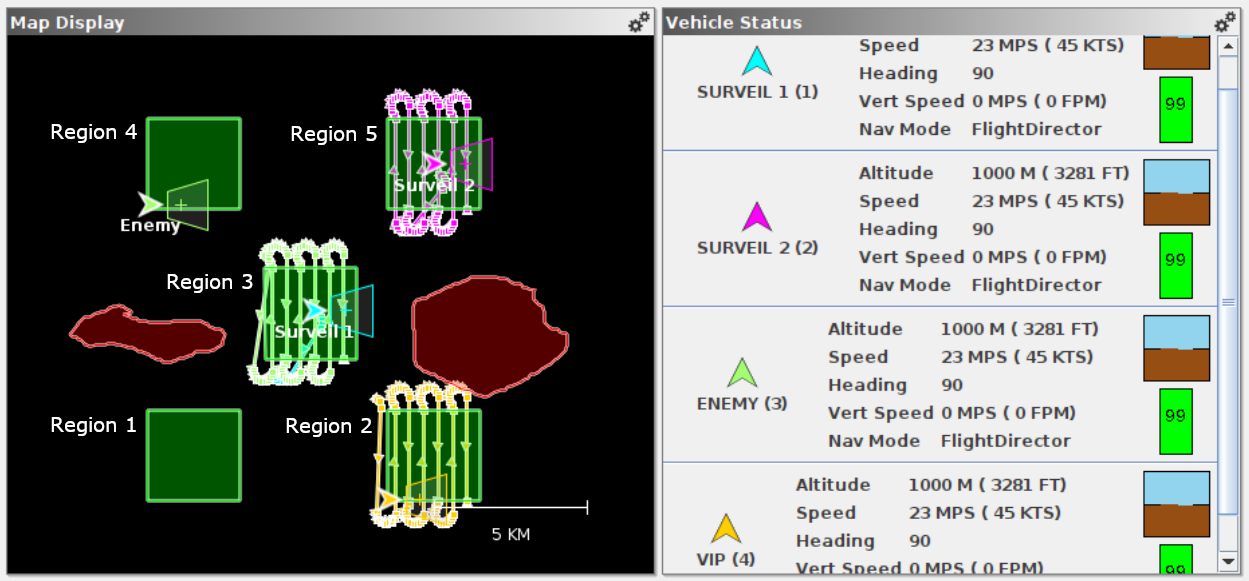
\includegraphics[width=\textwidth]{smallMission}
  \caption{A VIP escort multi-UAV mission as simulated in OpenAMASE using a Salty-synthesized controller that issues commands to the UAVs through OpenUxAS.}
  \label{fig:vipEscort}
\end{figure}

A particular instantiation of this mission is shown in \figref{fig:vipEscort}, as depicted in 
the open source Aerospace Multi-Agent Simulation Environment (OpenAMASE)\footnote{https://github.com/afrl-rq/OpenAMASE}. 
It includes the VIP, two surveillance UAVs numbered 1 and 2, one enemy UAV, and five regions numbered 1 to 5. 
Environment inputs include integer variable $loc_e \in \{1 \dots 5\}$, which encodes the current region of the enemy UAV, 
and Boolean variables $sr_i$ for $i = \{1 \ldots 5\}$, where $sr_i$ is true if and only if region $i$ has been visited at some point by a surveillance UAV. 
% Note that here, we assume surveillance of a region occurs if and only if a surveillance UAV has been in that region. 
System outputs include integer variables $loc_v, loc_{s1}, loc_{s2} \in \{1 \dots 5\}$, which indicate the current region of the 
VIP and surveillance UAVs 1 and 2, and Boolean variables $vTrack_1$ and $vTrack_2$, which indicate whether surveillance UAVs 1 and 2 
are executing a behavior to follow the VIP. 
Note that low-level control, e.g. waypoint planning and sensor steering, 
is implemented by the open source Unmanned Systems Autonomy Services (OpenUxAS)\footnote{https://github.com/afrl-rq/OpenUxAS}. 
The controller synthesized by Salty implements high-level decision logic, 
and OpenUxAS monitors the state of the controller and translates its current output values to a set of UAV commands that are simulated in OpenAMASE.
For example, when $loc_v$ changes value to 2, OpenUxAS commands the VIP to follow a path from its current region to region 2, 
or when $vTrack_1$ changes from false to true, OpenUxAS commands surveillance UAV 1 to fly next to the VIP. 
The high-level controller synthesized by Salty makes some assumptions about the low-level behaviors implemented by OpenUxAS, 
in this case, mainly that all UAVs move at the same speed and transition to new regions at the same time. 
A workflow for connecting Salty-implemented controllers with OpenUxAS and OpenAmase is described in \cite{elliott2019salty}, 
and all of the scripts, configuration files, etc. needed to run this example are available on the Salty repository.


%Note that all UAVs are assumed to move synchronously, 
%i.e. if any change regions, the change happens at the same time.

For this mission, the GR(1) specifications for the environment are:
%
\small
\begin{align}
\varphi_e^i  = & \;\; (loc_e = 4) \land \lnot sr_1 \land \lnot sr_2 \land sr_3 \land \lnot sr_4 \land sr_5  \label{eq:vipEnvInit} \\
\varphi_e^t  = & \bigwedge_{i = \{1 \ldots 5\}} \always \Big((loc_{s1} = i) \lor  (loc_{s2} = i) \limplies \lnext sr_i \Big) \land \mbox{} \label{eq:srSet} \\
 & \bigwedge_{i = \{1 \ldots 5\}} \always \Big(\big(\lnot (loc_{s1} = i) \land  \lnot (loc_{s2} = i) \land \lnot sr_i \limplies \lnext \lnot sr_i\big) \land \mbox{} \label{eq:vipEnvNoSp} \\
 & \quad\quad\quad\quad\quad \big(sr_i \limplies \lnext sr_i\big)\Big) \land \mbox{} \label{eq:vipEnvSetSp} \\
% &  \bigwedge_{i = \{1 \ldots 5\}} \always  \big(sr_i \limplies \lnext sr_i\big) \land \mbox{} \label{eq:vipEnvSetSp} \\
 & \;\; \always \lnot (loc_e = 1) \land \always \lnot (loc_e = 2) \label{eq:vipEnvDisallowedRegions} \\
\varphi_e^l = & \;\; \always \eventually \lnot (loc_e = 3) \land \always \eventually \lnot (loc_e = 4) \land \always \eventually \lnot (loc_e = 5). \label{eq:vipEnvLiveness}
\end{align}
%
These express \eqnref{eq:vipEnvInit} that the enemy UAV starts in region 4, and regions 3 and 5 start as surveilled; 
\eqnref{eq:srSet} that a region is considered to be surveilled after either one of the surveillance UAVs is in it; 
\eqnref{eq:vipEnvNoSp} that a previously unsurveilled region remains unsurveilled if neither surveillance UAV is in it; 
\eqnref{eq:vipEnvSetSp} that once a region is surveilled, it remains surveilled; 
\eqnref{eq:vipEnvDisallowedRegions} that the enemy UAV cannot go to regions 1 or 2; and
\eqnref{eq:vipEnvLiveness} that the enemy UAV must infinitely often not be in each region 3, 4, and 5. 


GR(1) specifications for the system are:
\small
\begin{align}
\varphi_s^i  = & \;\; (loc_v = 2) \land (loc_{s1} = 3) \land (loc_{s2} = 5) \land \lnot vTrack_1 \land \lnot vTrack_2 \label{eq:vipSysInit} \\
\varphi_s^t  =  & \quad\quad\quad\quad\; \always \Big( \lnot(loc_v = \lnext loc_v) \limplies (\lnext vTrack_1 \lor \lnext vTrack_2) \Big)  \land \mbox{} \label{eq:vipNoMoveUnlessTracked} \\
 & \;  \bigwedge_{i = \{1 \ldots 2\}} \;\;   \always \Big(vTrack_i \limplies (sloc_i = loc_v)\Big) \land \mbox{} \label{eq:vipSysVtrack} \\
& \; \bigwedge_{i = \{1 \ldots 5\}} \;\;   \always \Big((loc_v = i) \limplies \lnot(loc_e = i)\Big) \land \mbox{} \label{eq:vipSysNoEloc} \\
 & \bigwedge_{i = \{v, s1, s2\}} \always \Big(\big( \lnext(loc_i = 1) \limplies (loc_i = 1) \lor (loc_i = 2) \lor (loc_i = 3)   \big) \land \mbox{} \label{eq:vipSysTrans1} \\
 & \quad\quad\quad\quad\quad\;\;\; \big(\lnext (loc_i = 2) \limplies (loc_i = 1) \lor (loc_i = 2) \lor (loc_i = 3)   \big) \land \mbox{} \label{eq:vipSysTrans2} \\
  & \quad\quad\quad\quad\quad\;\;\; \big(\lnext (loc_i = 3) \limplies \bigvee_{j=\{1\ldots5\}} (loc_i = j) \big) \land \mbox{}  \label{eq:vipSysTrans3} \\
%  & \quad\quad\quad\quad\quad\;\;\; \big((loc_i = 3) \limplies (loc_i = 1) \lor (loc_i = 2) \lor (loc_i = 3) \lor \mbox{} \nonumber \\ 
%  & \quad\quad\quad\quad\quad\quad\quad\quad\quad\quad\quad\quad     (loc_i = 4) \lor (loc_i = 5)   \big) \land \mbox{} \nonumber \\
  & \quad\quad\quad\quad\quad\;\;\; \big(\lnext (loc_i = 4) \limplies (loc_i = 3) \lor (loc_i = 4) \lor (loc_i = 5)   \big) \land \mbox{} \label{eq:vipSysTrans4} \\
  & \quad\quad\quad\quad\quad\;\;\; \big(\lnext (loc_i = 5) \limplies (loc_i = 3) \lor (loc_i = 4) \lor (loc_i = 5)  \big)  \Big)  \label{eq:vipSysTrans5} \\
\varphi_s^l = & \;\; \always \eventually (loc_v = 1) \land \always \eventually (loc_v = 5). \label{eq:vipSysLiveness}
\end{align}
%
These express \eqnref{eq:vipSysInit} that the VIP starts in region 2, surveillance UAV 1 in region 3, and surveillance UAV 2 in region 5; 
\eqnref{eq:vipNoMoveUnlessTracked} that the VIP does not change regions unless a surveillance UAV is tracking it; 
\eqnref{eq:vipSysVtrack} that a surveillance UAV can only track the VIP if they are in the same region at the same time; 
\eqnref{eq:vipSysNoEloc} that the VIP cannot be in the same region as the enemy UAV at the same time; 
\eqnref{eq:vipSysTrans1} and \eqnref{eq:vipSysTrans2} that the VIP and surveillance UAVs can move from regions 1 or 2 to regions 1, 2, or 3;
\eqnref{eq:vipSysTrans3} that the VIP and surveillance UAVs can move from region 3 to any other region; 
\eqnref{eq:vipSysTrans4} and \eqnref{eq:vipSysTrans5} that the VIP and surveillance UAVs can move from regions 4 or 5 to regions 3, 4, or 5; 
and \eqnref{eq:vipSysLiveness} that the VIP must go to regions 1 and 5 infinitely often.

We have chosen to describe this particular example in detail because during the process of extending Salty to produce SPARK translations, 
we discovered a previously undetected problem with this example's specification. 
As written, the specification is realizable and produces what appears at a glance to be a reasonable controller with 97 states. 
In fact, we had previously run this example with OpenAMASE, OpenUxAS, and a Python controller synthesized by Salty. 
However, we did not originally notice in the Python implementation that 34 of the controller's 97 states do not have successors. 
Since no special logic was added to Salty to handle this situation, the generated SPARK code included empty case statement alternatives in the \lstinline{Move} procedure. 
For example, in state 2 the case statement alternative is simply \lstinline{when 2 =>}, with no statements in the body. 
This code failed to compile, since SPARK does not allow for fall-through behavior in case statements (nor does Ada); 
explicit statements are expected for each case statement alternative. 
In Python, this error went undetected; 
the transition relation for the controller is encoded as a map, and entries corresponding to states without successors 
simply had an empty list of ``next state'' values. 
We briefly note that if we had encoded the controller using a map in SPARK, 
the error would still have been detected through SPARK analysis rather than a syntactic check of the code; 
the case statement encoding was chosen for efficiency reasons to be discussed in \sectref{sec:lessonsLearned}.

This error is the result of a subtlety of the semantics of GR(1) specifications. 
Recall that GR(1) specifications take the form $\varphi_e \limplies \varphi_s$. 
Obviously a specification of this form is satisfied if $\varphi_e$ and $\varphi_s$ are both true, 
but it is also satisfied if $\varphi_e$ is false. 
Also recall from the introduction that GR(1) specifications are interpreted in the context of a two-player game 
in which the environment takes its turn first and the system takes its turn second. 
The issue here is that the environment is able to take transitions that will necessarily cause it to violate $\varphi_e^t$ in the next time step. 
Note that $\varphi_e^t$ contains terms of the form $\always \lnot p$, specifically $\always \lnot (loc_e = i)$ for $i = \{1, 2\}$  \eqnref{eq:vipEnvDisallowedRegions}. 
Note that a term of the form $\always \lnot p$ is not the same as a term of the form $\always \lnext \lnot p$. 
The distinction is important. 
If the environment chooses $p$ for the ``next'' time step, this does not violate $\always \lnot p$ in the ``current'' time step. %, since the new ``current'' time step is only constructed once the environment and system have both taken their turn. 
However, once the next state is reached, $p$ becomes the new ``current'' value, and $\always \lnot p$ 
will now be violated no matter what the environment chooses.
Generally, specifications should follow the latter form $\always \lnext \lnot p$, 
which prohibits the environment from choosing $p$ in the ``next'' time step. 
This was indeed an error in these specifications, so we changed $\always \lnot (loc_e = 1) \land \always \lnot (loc_e = 2)$
 to $\always \lnext \lnot (loc_e = 1) \land \always \lnext \lnot (loc_e = 2)$ in \eqnref{eq:vipEnvDisallowedRegions}.
However, we also modified Salty to \lstinline{raise Program_Error} in cases with no successors 
and checked that we were still able to prove $\varphi_e \limplies \varphi_s$ 
(since reaching these cases would require violating the precondition $\varphi_e$). 
Such cases amount to instances in which the precondition on \lstinline{Move} is would have to be violated, which is why we allow the user to execute \lstinline{Env_Trans} 
as discussed in \sectref{sec:implementation}. 
We also plan to have Salty issue a warning when there are states with no successors, 
since such cases are likely unintended by the user.


%%%%%%%%%%%%%%%%%%%%%%%%%%%%%%%%%%%%%%%%%%%%%%%%%%%%%%%%%%%%%%%%%%%%%%%%%%%%%%%%
% CASE STUDIES
%%%%%%%%%%%%%%%%%%%%%%%%%%%%%%%%%%%%%%%%%%%%%%%%%%%%%%%%%%%%%%%%%%%%%%%%%%%%%%%%
\section{Results}
\label{sec:caseStudies}

To further evaluate the utility and feasibility of our approach, we pulled additional example GR(1) specifications from a variety of sources including 
Anzu, LTLMoP, TuLiP, Slugs, and Salty, all of which make their examples publicly available for download. 
GR(1) specifications in Salty format, synthesized SPARK packages, and SPARK analysis results for all of these examples are available on the 
Salty GitHub repository, including the traffic light example of the previous section. 
We note that while some examples are small and simple, e.g. demos along the lines of the traffic light example, 
there are many in our collection that are more realistic. 
For instance, Anzu has controller specifications for a generalized IBM buffer and an AMBA bus. 
LTLMoP and TuLiP have specifications for robot controllers that have been demonstrated on simulated and/or real robots. 
And Salty has specifications for controllers to coordinate the actions of teams of vehicles that have been demonstrated in simulation. 

\figref{fig:timingResults} shows the amount of time needed to analyze examples as a function of total number of transitions 
in the Moore machine representing the controller, 
with examples that could not be analyzed due to memory errors set to 1. 
Results were generated on a Linux VM given 24GB RAM and 4 processors on a MacBook Pro with a 2.9 GHz Intel Core i9 with 32GB RAM.
We ran 40 examples in total. 
Results for 33 examples are plotted. 
On most examples with less than 4000 transitions, 
SPARK was able to completely verify or prove the generated code complies with its specification. 
Examples that had more than 4000 transitions (the 7 unplotted examples) required too much memory to analyze, 
resulting in errors when attempting to verify them in SPARK. 

Of examples with less than 4000 transitions, two resulted in errors. 
These two examples had abnormally large specifications consisting of approximately 1000 atomic propositions each, 
whereas most other examples with a similar number of transitions had 500 or less. 
Such cases occur, e.g. when systems include a large number of inputs and/or outputs but have very tight specifications on 
how they can transition, leading to large specifications and therefore lengthy pre- and postconditions but relatively small controllers.

Two examples with less than 4000 transitions could only be partially proven. 
One was relatively large, with about 2000 transitions. 
The other had arithmetic terms in its specification (Salty and Slugs support integer inputs and outputs); 
we are investigating why this example does not fully prove, 
since we feel that SPARK should be capable of fully proving this example.



\begin{figure}
\includegraphics[width=\textwidth]{salty_log.eps}
\caption{Timing results for example SPARK controllers as a function of number of transitions in the controller. ``Proven'' examples were fully verified, ``partial'' examples were partially verified, and ``error'' examples were too big to analyze.}
\label{fig:timingResults}
\end{figure}

\vspace{-1em}

%%%%%%%%%%%%%%%%%%%%%%%%%%%%%%%%%%%%%%%%%%%%%%%%%%%%%%%%%%%%%%%%%%%%%%%%%%%%%%%%
% Lessons Learned
%%%%%%%%%%%%%%%%%%%%%%%%%%%%%%%%%%%%%%%%%%%%%%%%%%%%%%%%%%%%%%%%%%%%%%%%%%%%%%%%
\section{Lessons Learned}
\label{sec:lessonsLearned}

Throughout the process of synthesizing and attempting to verify controllers in SPARK, we learned several lessons, 
both about SPARK and about some of the finer points of GR(1) specifications.

In terms of encoding SPARK controllers for verification, we originally tried to 
mirror the approach taken in other Salty language targets by building a static lookup table for state transitions. 
To do this, we tried to create an array of \lstinline{Formal_Hashed_Maps} indexed by \lstinline{State_Num}, where keys 
were derived from environment input values and used to look up the next \lstinline{State_Num} and corresponding system output values. 
Ghost functions consisting of nested quantified expressions were used to check that in each state, specification properties held 
using input and output values encoded by the current state and all states reachable as contained in the hashed maps.
These functions comprised the post-condition of a function that initialized the controller's lookup table. 
The body of the \lstinline{Move} procedure simply retrieved the outputs and next state from the lookup table 
using its stored \lstinline{State_Num} and \lstinline{Environment} input.
The public portion of the SPARK specification was largely unchanged.
This approach was only able to prove the smallest of examples in a reasonable amount of time. 

While the use of formal containers was intuitive, they are more complex to reason about with respect to proof 
because they require reasoning about models of the containers. 
Encoding the lookup table as a case statement is more straightforward, because for instance, 
it is ``obvious'' to the underlying solvers that state transitions are static and that a transition exists for every possible input, since 
case statements must be exhaustive. 
%When building a lookup table represented as a formal container, one can imagine the provers would have to do additional reasoning 
%to ensure that all possible transitions are defined for each state, and no entries are ever deleted or added to the container at other points in the code. 
Encoding the \lstinline{Move} procedure as a case statement still has some issues, mainly that 
(1) the generated code can be quite long, leading to memory errors when trying to prove the subprogram with SPARK, and
(2) since the solvers prove all case statement alternatives at the same time and the number of case statement alternatives grows 
exponentially with the number of inputs, sometimes the solvers are not able to prove the postcondition.
A solution to both problems could be to split the \lstinline{Move} procedure into several smaller procedures. %, e.g. splitting on the number of states 
% in a manner similar to a classic programmer splitting large subprograms into smaller ones. 
This would allow SPARK to apply modular analysis on several smaller procedures, thus enabling the proof on larger files. 
We are currently investigating ways to split up the procedure that does not accidentally create more difficulties for the underlying solvers.

The process of encoding and analyzing controllers in SPARK did reveal some unexpected behaviors. 
First, as discussed in \sectref{sec:vipExample}, there were two example controllers\footnote{Salty's vip\_orig.salt and Anzu's arbiter.salt} 
with specifications that resulted in states with no successors. 
As a result, these controllers contained empty case statements in the \lstinline{Move} procedure. 
We had previously run the Salty-synthesized controller in Python for the example in \sectref{sec:vipExample} and had not noticed the error, 
though it would have resulted in an unhandled runtime exception if one of the states without successors had been reached.  
Second, a meta-analysis of SPARK timing results also revealed that other examples in our database did not have any inputs, 
i.e. they amounted to synthesizing a system independent of an environment. 
In those cases, we had specifications for a non-existent environment that were vacuous, 
and this was causing SPARK to take an abnormally long amount of time to verify these controllers, given their relatively small size. 
These controllers did not have errors per se, 
but they were inefficiently encoded. 
We plan to modify Salty to handle such cases by removing the environment, functions over the environment, and
all references to the environment in all pre- and postconditions.
This greatly decreases verification time and also reduces the size and increases the efficiency of the code.

%%%%%%%%%%%%%%%%%%%%%%%%%%%%%%%%%%%%%%%%%%%%%%%%%%%%%%%%%%%%%%%%%%%%%%%%%%%%%%%%
% CONCLUSIONS
%%%%%%%%%%%%%%%%%%%%%%%%%%%%%%%%%%%%%%%%%%%%%%%%%%%%%%%%%%%%%%%%%%%%%%%%%%%%%%%%
\section{Conclusions}
\label{sec:conclusions}

We were able to successfully use SPARK to verify safety and transition properties of moderately sized controllers 
synthesized by Salty from GR(1) specifications. 
Encoding the controllers and all of the annotations necessary for these controllers to prove automatically was relatively straighforward, 
and it was satisfying to be able to generate proofs using a single tool rather than having to use multiple tools to perform verification.
Furthermore, the act of performing ``end-to-end'' verification with SPARK on such controllers was valuable because (1) it revealed a type of specification error in some examples that would result in  runtime errors in other Salty target languages, and (2) it revealed cases in which controllers were inefficiently encoded, i.e. when there is no environment.



In terms of future work, we can potentially improve the scalability of our approach by decomposing the \lstinline{Move} procedure 
into several subprocedures, as discussed in the previous section. 
We are also interested in expressing and proving liveness properties. 
Liveness properties will be more challenging to verify because they necessarily require reasoning about future states beyond the ``next'' state. 
Verifying system liveness in SPARK will require something like encoding a lookahead buffer and showing that certain states will inevitably be reached 
when the environment satisfies its specification, which can itself also include liveness terms. 
This is likely to result in complex first-order formulas with alternating quantification over time, which are 
notoriously hard to handle in automated solvers, so discharging the resulting proof obligations may prove to be a challenge.
To tackle this issue, collaboration with a model checker performing verification at the level of the input language might be more appropriate.

%
% ---- Bibliography ----
%
% BibTeX users should specify bibliography style 'splncs04'.
% References will then be sorted and formatted in the correct style.
%
\newpage
\bibliographystyle{splncs04}
\bibliography{bibfile}

\end{document}
